\section{Recuperação de Informação} \label{sec:RecuperaçãoInformação}
% Falar da recuperação de informação com conceito humano

% Estrutura

% - Histórico de RI, explicando o surgimento de métodos de RI com as bibliotecas

A procura por informação é uma necessidade das pessoas, e um dos modos primordiais de assim fazer é consultar outras pessoas por informação.
No entanto, devido ao grande acúmulo de informação das sociedades, uma pessoa não pode carregar consigo todo o conhecimento da humanidade.
Assim, um modo considerado primordial de transferir esse conhecimento, que tratamos aqui como informação, é por meio de registros físicos em papel, livros e similares \cite[p.~1]{Grossman2004IRAH}.

No intuito de organizar esses diversos livros, artigos e afins é notória a função dos bibliotecários em separar os diversos tipos de conhecimento que os mais diversos livros podem abrigar e, portanto, os sistemas de classificação de áreas e subáreas do conhecimento são um auxílio para as necessidades de busca por informação que uma pessoa pode ter \cite[p.~1]{Manning2008IIR} \cite[p.~1446]{Sanderson2012THIRR} \cite[p.~6]{Baeza-Yates1999}. 
Esses sistemas de classificação facilitam a localização de informações específicas a partir de uma pergunta que uma pessoa pode fazer, mas é necessário o conhecimento de como o sistema de classificação funciona para que o usuário possa tentar saciar sua necessidade, ou pelo menos será preciso de um especialista no sistema (o bibliotecário) para lhe guiar.
E mesmo assim, depois de adquirir os diversos materiais que podem responder à sua pergunta, esta pessoa ainda terá que conferir nos textos se estes satisfazem sua necessidade.

% - RI em equipamentos eletromecânicos no início do século 20
% -- O que fez surgir esses sistemas, a necessidade

Esses sistemas de classificação manual se mostram bem ineficazes devido ao surgimento crescente constante de novas informações \cite[p.~6]{Baeza-Yates1999} desde o início do século 20. 
Temos assim uma imensidão de novas pesquisas científicas sendo publicadas, livros surgindo, entre outros registro históricos, que precisam ser classificados, mas existe também o problema da classificação não poder abranger todo tipo de necessidade que tal material pode satisfazer \cite[p.~1444]{Sanderson2012THIRR}. 
A preocupação com sistemas que possam indexar todo esse material e fornecer um acesso rápido às necessidades de informação de uma pessoa surgiu também no início do século 20 \cite{Bush:1979:WMT:1113634.1113638}, onde sistemas mecânicos de recuperação de informação foram visionados.


% - A área de pesquisa de RI que surgiu com a utilização de computadores para indexar informação
% -- A utilização de computadores para fazer o serviço de RI

A partir da criação de sistemas computacionais na década de 1940, foi vista a possibilidade de criação de sistemas que armazenassem informações e possibilitassem essa consulta rápida sobre as informações armazenadas, sendo necessários estabelecer algoritmos que retornassem informação relevante ao que o usuário do sistema procura. 
Tendo então nesse momento o início do campo científico de Recuperação de Informação (\textit{Information retrieval}, IR) que é encontrar material (geralmente documentos) de natureza desestruturada (geralmente texto) que satisfaça uma necessidade de informação dentro de grandes acervos (geralmente armazenados em computadores) \cite[p.~1]{Manning2008IIR}.

A lei de Moore diz que o crescimento da velocidade de processamento é contínua, e similarmente existe uma duplicação constante da capacidade de armazenamento digital a cada dois anos. % CARECE DE FONTES - Preciso procurar
Logo, a necessidade de sistemas de Recuperação de Informação surge do crescimento exponencial das coleções de informação derivadas do crescimento de armazenamento, e consequente inabilidade das técnicas tradicionais de catalogação de lidar com isso \cite{Sanderson2012THIRR}.
Ter um amontoado de conhecimento, informação, e não poder acessar o que é relevante de modo rápido não é interessante pois assim o desenvolvimento de pesquisas, por exemplo, fica comprometido e pode perder relevância \cite{Bush:1979:WMT:1113634.1113638}.

% -- Conceitos fundamentais de RI
A RI como uma disciplina de pesquisa se iniciou no final da década de 50 com o início do uso de computadores para procurar referências de texto associadas com um assunto \cite[p.~3]{Sanderson2012THIRR}, as preocupações iniciais dessa área são 
\begin{enumerate*}[label=(\alph*)]
\item \textit{como indexar documentos} e \item \textit{como recuperá-los},
\end{enumerate*}
sendo a busca como melhor fazer essas tarefas o objetivo da RI.

Logo no início do seu desenvolvimento as técnicas de RI buscaram se basear em sistemas existentes já consolidados no campo bibliotecário para indexar coleções de itens, tendo como uma técnica de abordagem clássica atribuir códigos numéricos a essas coleções, como por exemplo o feito pelo sistema de Classificação Decimal de Dewey \cite[p.~1446]{Sanderson2012THIRR}.
No entanto foi demonstrado por \citeonline{Cleverdon1959TESUIR} que um sistema baseado em palavras, como o sistema Uniterm proposto por \citeonline{Taube1952UTCI}, era tão bom e até melhor que outras abordagens clássicas, sendo a indexação por palavras posteriormente adotada pelos sistemas de RI \cite[p.~1446]{Sanderson2012THIRR}.

\begin{figure}[h]
    \centering
    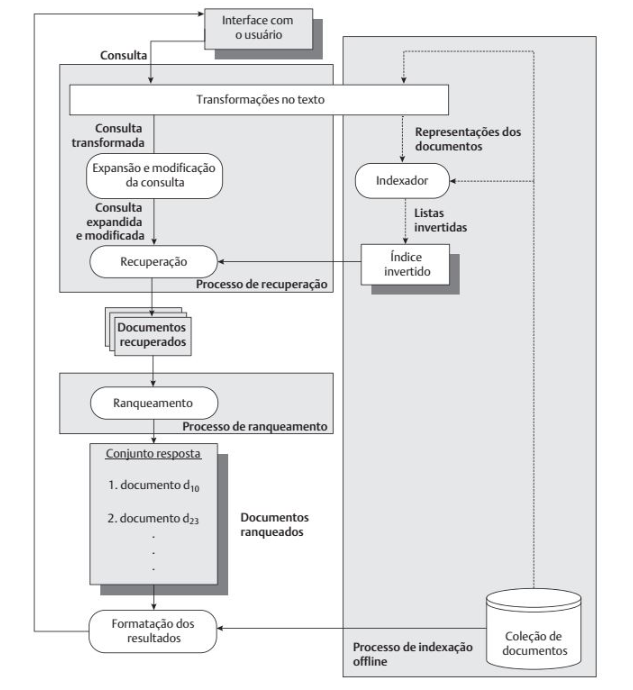
\includegraphics[width=0.85\textwidth]{img/baeza2013-figura-1-3.png}
    \caption{Processos de indexação, recuperação, e ranqueamento dos documentos. Figura extraída de \citeonline[p.~8]{Baeza-Yates2011}.}
    \label{fig:diagrama-baeza2013-fig1-3}
\end{figure}

Um exemplo do funcionamento de um sistema moderno de RI pode ser visto na Figura \ref{fig:diagrama-baeza2013-fig1-3}, onde está apresentado um fluxograma dos processos de indexação, recuperação, e ranqueamento de documentos. 
Sendo o ranqueamento de sistemas de RI o nosso interesse neste trabalho, alguns dos termos apresentados nessa Figura serão abordados logo mais.

% -- Os primeiros sistemas de RI, booleanos 
\subsection{Métodos booleanos} \label{subsec:MétodosBooleanos}

    Uma consulta (chamada de \textit{query}) representa uma necessidade de informação a ser saciada por um sistema de RI, e essa consulta é composta de termos (um sinônimo para palavras) que nos primeiros desses sistemas era limitada a combinações lógicas e eram recuperados os documentos que tinham correspondência exata com ela \cite[p.~1446]{Sanderson2012THIRR}. 
    Este método de recuperação de informação é conhecido como recuperação booleana, e para indexar os documentos é utilizada, geralmente, uma matriz binária de incidência de termo-documento. 
    Exemplificamos uma matriz dessas na Tabela \ref{tab:matriz-incidência-termo-documento}, que é o exemplo dado por \citeonline[p.~3--4]{Manning2008IIR} de uma matriz de incidência de termo-documento para o livro \textit{Shakespeare’s Collected Works}, que reúne as obras completas de Shakespeare.

    \begin{table}[H]
    \centering
    \caption{Matriz de incidência de termo-documento do livro \textit{Shakespeare’s Collected Works}. Cada elemento (i, j) da matriz é 1 se a peça de teatro na coluna j contém a palavra na linha i, caso contrário o elemento é 0.}
    \begin{adjustbox}{max width={\textwidth},keepaspectratio}%
    \begin{tabular}{|c|c|c|c|c|c|c|c}
        \hline
        \diagbox{Palavra}{
            \raisebox{-1.27cm}{
                \rotatebox{90}{
                    \parbox{1.6cm}{\centering Peça \\ de teatro}
                }
            }
        } 
        & \makecell{Antony \\ and \\ Cleopatra} 
        & \makecell{Julius \\ Caesar} 
        & The Tempest 
        & Hamlet 
        & Othello 
        & Macbeth 
        & ... 
        \\ \hline
        Antony     & 1 & 1 & 0 & 0 & 0 & 1 & \\
        Brutus     & 1 & 1 & 0 & 1 & 0 & 0 & \\
        Caeasar    & 1 & 1 & 0 & 1 & 1 & 1 & \\
        Calpurnia  & 0 & 1 & 0 & 0 & 0 & 0 & \\
        Cleopatra  & 1 & 0 & 0 & 0 & 0 & 0 & \\
        mercy      & 1 & 0 & 1 & 1 & 1 & 1 & \\
        worser     & 1 & 0 & 1 & 1 & 1 & 0 & \\
        ...        & & & & & & & 
    \end{tabular}
    \end{adjustbox}
    \legend{\ABNTEXfontereduzida \textbf{Fonte:} Tabela adaptada de \citeonline[p.~4]{Manning2008IIR}.}
    \label{tab:matriz-incidência-termo-documento}
\end{table}
% \clearpage

% -- A pesquisa de RI sendo desenvolvida, citar sistemas rankeados
\subsection{Ranqueamento} \label{subsec:Ranqueamento}
Devido à limitação dos métodos booleanos de somente retornar resultados conforme a presença ou não dos termos da consulta nos documentos \cite[p.~100]{Manning2008IIR}, foi proposto em 1957 por Luhn e 1959 por Maron \textit{et al.} uma abordagem de recuperação ranqueada \cite[p.~1446]{Sanderson2012THIRR} a qual, em contraste com recuperação booleana, baseada nos termos de consulta estabelecia uma pontuação para cada artigo de modo probabilístico e retornava os artigos de modo ordenado e demonstraram que essa técnica sobressaía a recuperação booleana.

% Explicar o funcionamento de uma recuperação ranqueada, como é feito esse ranqueamento?
O procedimento fundamental para ranqueamento dos documentos, conforme os termos de consulta, consiste na atribuição de pontuação aos documentos a partir da contabilização do número de aparições (chama de frequência) de cada um dos termos no documento.
Essa pontuação é calculada considerando que além da frequência do termo, denotada como $\text{tf}_{\text{\textit{t},\textit{d}}}$ que é o número de ocorrências do termo \textit{t} em um documento \textit{d}, existe também a sua relevância, que depende do número de aparições do termo na coleção de documentos inteira.
Quanto mais um termo aparece na coleção menos relevante ele é, e este valor de relevância é denotado por $\text{idf}_{\text{\textit{t}}}$ que é o inverso da frequência de um termo \textit{t} em uma coleção de documentos.
Segundo \citeonline[p.~108]{Manning2008IIR} este valor da relevância é calculado do seguinte modo:

\begin{equation}
    \text{idf}_{\text{\textit{t}}} = \log{\frac{N}{\text{df}_{\text{\textit{t}}}}}.
\end{equation}

O valor resultante da relação entre a frequência do termo e o inverso da frequência nos documentos é chamado de $\text{tf-idf}_{\text{\textit{t},\textit{d}}}$ (\textit{term frequency-inverse document frequency}), sendo este valor um dos pesos mais utilizados para ranqueamento \cite[p.~107--110]{Manning2008IIR}, e é calculado  como segue:
\begin{equation}
    \text{tf-idf}_{\text{\textit{t},\textit{d}}}  = \text{tf}_{\text{\textit{t},\textit{d}}} \times \text{idf}_{\text{\textit{t}}}.
\end{equation}

\begin{table}[h]
    \centering
    \begin{tabular}{|l|r|r|r|r|r|r|r|r|}\hline
         \multicolumn{3}{|c|}{\diagbox{Termo}{\raisebox{-1.87cm}{\rotatebox{90}{\parbox{1.6cm}{\centering Documento}}}}} & \multicolumn{2}{|c|}{Doc1} & \multicolumn{2}{|c|}{Doc2} & \multicolumn{2}{|c|}{Doc3} \\ \hline
                    & $\text{df}_{\text{\textit{t}}}$ & $\text{idf}_{\text{\textit{t}}}$ & $\text{tf}_{\text{\textit{t},\textit{d}}}$ & $\text{tf-idf}_{\text{\textit{t},\textit{d}}}$ & $\text{tf}_{\text{\textit{t},\textit{d}}}$ & $\text{tf-idf}_{\text{\textit{t},\textit{d}}}$ & $\text{tf}_{\text{\textit{t},\textit{d}}}$ & $\text{tf-idf}_{\text{\textit{t},\textit{d}}}$ \\ \hline
         car        & 18165 & 1,65 & 27 & 44,55 & 4 & 6,6 & 24 & 39,6 \\
         auto       & 6723 & 2,08 & 3 & 6,24 & 33 & 68,64 & 0 & 0 \\
         insurance  & 19241 & 1,62 & 0 & 0 & 33 & 54,46 & 29 & 46,98 \\
         best       & 25235 & 1,5 & 14 & 21 & 0 & 0 & 17 & 25,5
    \end{tabular}
    \caption{Exemplo de cálculo do valor de tf-idf baseado nas tabelas disponível em \citeonline[p.~109--110]{Manning2008IIR}.}
    \label{tab:exemplo-tf-idf}
\end{table}

Na Tabela \ref{tab:exemplo-tf-idf} temos um exemplo de cálculo dos valores de tf-idf para posterior cálculo da pontuação para ranqueamento, conforme alguma determinada consulta. 
A pontuação de um documento \textit{d} é a soma dos pesos de tf-idf de cada termo \textit{t} em \textit{d}, sendo os termos \textit{t} presentes na consulta realizada \cite[p.~109]{Manning2008IIR}, representamos esse cálculo do seguinte modo:

\begin{equation}
    \label{eq:pontuação-simples-tf-idf}
    \text{Pontuação(\textit{q},\textit{d})} = \sum_{\textit{t} \in \textit{q}}^{} \text{tf-idf}_{\text{\textit{t},\textit{d}}}.
\end{equation}

% Quando uma consulta é feita são utilizados os valores 
% (onde Pontuação({\textit{auto},\textit{car}},DocX))  

Utilizando a Equação \ref{eq:pontuação-simples-tf-idf} uma consulta com os termos \textit{auto car} retornaria no seu ranqueamento os documentos com a seguinte pontuação, calculamos Pontuação(\{\textit{auto},\textit{car}\},DocX) para cada documento, por exemplo:
\begin{itemize}
    \setlength\itemsep{-0.2em}
    \item Doc1: 50,79
    \item Doc2: 75,24
    \item Doc3: 39,60
\end{itemize}

A ordenação dos documentos apresentados como resultado à consulta \textit{auto car} seria então a seguinte: 1\textordmasculine{} - Doc2; 2\textordmasculine{} - Doc1; e 3\textordmasculine{} - Doc3, que se observamos a Tabela \ref{tab:exemplo-tf-idf} é um bom resulto já que o Doc2 contém uma grande frequência do termo \textit{auto} e o Doc3 não possui este termo.


Ao longo dos anos foi demonstrada a superioridade da recuperação ranqueada sobre a recuperação booleana \cite{Jones:1981:IRE:539571}, e são as técnicas de recuperação ranqueadas que trazem maior interesse para a área de Mineração de Textos, em específico estamos interessados nos modelos vetoriais e os modelos probabilísticos de RI que são evoluções da recuperação ranqueada.
% ESTOU PENSANDO EM JÁ CITAR O BM25 no parágrafo acima.
% -- Em algum ponto mencionar que Recuperação de Informação (Information Retrieval) não deve ser confundido com Procura de Informação (Information Search), pois a Procura de Informação é o campo que estuda a interação das pessoas com sistemas de recuperação de informação.


% TESTE DE SIGLAS
\nomenclature{Fig.}{Figura TTTTT}
\nomenclature{$A_i$}{Area of the $i^{th}$ component}
\nomenclature{456}{Isto éum número}
\nomenclature{123}{Isto éoutro número}
\nomenclature{a}{primeira letra do alfabeto}
\nomenclature{lauro}{este émeu nome}